\chapter{``Quantum" Behaviour}

\section{Macroscopic Quantum Scale Behaviors} 
	    \subsubsection{Basic Parameters}
	       Consider a fluid of density $\rho$, viscosity $\nu$, and surface tension $\sigma$, in a bath of depth $H$ driven vertically at an amplitude $A_0$ at frequency $f=\omega/{2\pi}$. By defining $\mathnormal{\gamma}=A_0\omega^2$, the effective gravity in the frame of reference of the bath is $g+\gamma~\mathrm{sin}(\omega t)$. 
	       
	   \begin{figure}[h]
	       \centering
	    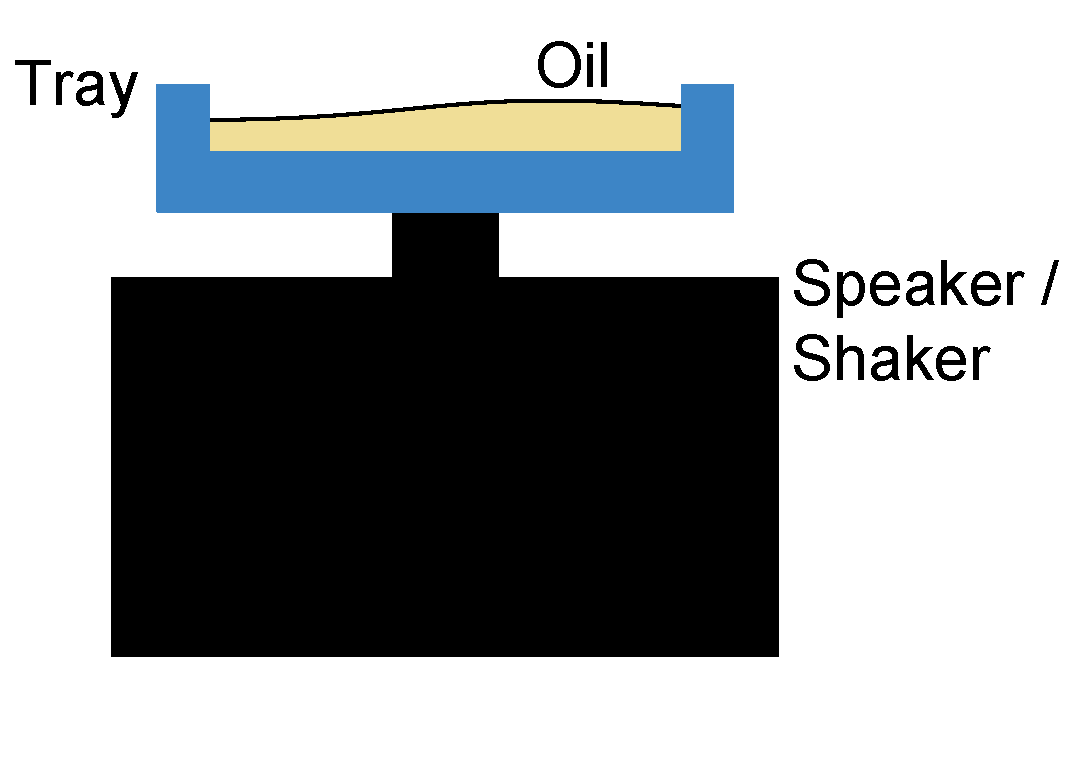
\includegraphics[scale=0.35]{HQASetup.pdf}
	     \caption{The experimental setup. The tray vibrates with an amplitude $A_0$.}
	 \label{regime}
	\end{figure}
	       
	       The oil droplet of diameter $D$ bounces in the regime $\gamma<\gamma_F$, where $\gamma_F$ is the Faraday threshold (at this point, Fraday waves appear). The important experimental limits are outlined in \refTab{approxlimits}. 
	       \begin{table}[htdp] 
\caption[Basic Table 1]{Approximate Limits for Bouncing Drop Behavior} 
\begin{center} 
\begin{tabular}{c c c} 
\toprule 
  Parameter &  Lower Limit & Upper Limit \\
  \midrule
Viscocity $\nu$ (cSt) & 10 & 100 \\ 
Bath Depth $H$ (mm) & 4 & 10 \\
Frequency $f$ (Hz) & 20 & 150 \\
Amplitude $A_0$ (mm) & 0.1 & 1 \\
Drop Diameter $D$ (mm) & 0.6 & 1.0 \\
\bottomrule 
\end{tabular}
\end{center}
\label{approxlimits} 
\end{table}	

For certain parameters, the bouncing drop will behave differently. The vibration number describes ``the relative magnitude of the forcing frequency and the drop's natural oscillation frequency," and is given by:
	       	      
\begin{equation} \label{vibrationnumber}
V_i = \frac{\omega}{2}\sqrt{\frac{\rho D^3}{2\sigma}}
\end{equation}   	       	       
	       	       The natural frequency of the droplet occurs around $V_i = 0.65$, where the droplet can exhibit both walking and bouncing behaviors. Setting up a plot with $V_i$ on the y axis and (dimensionless) ${\gamma}/{g}$ on the x axis can help in showing the behavior of the droplet, shown in \refFig{regime}. 
	    
	    \begin{figure}[h]
	% the options are h = here, t = top, b = bottom, p = page of figures.
	% you can add an exclamation mark to make it try harder, and multiple
	% options if you have an order of preference, e.g.
	% \begin{figure}[h!tbp]
	   
	       \centering
	    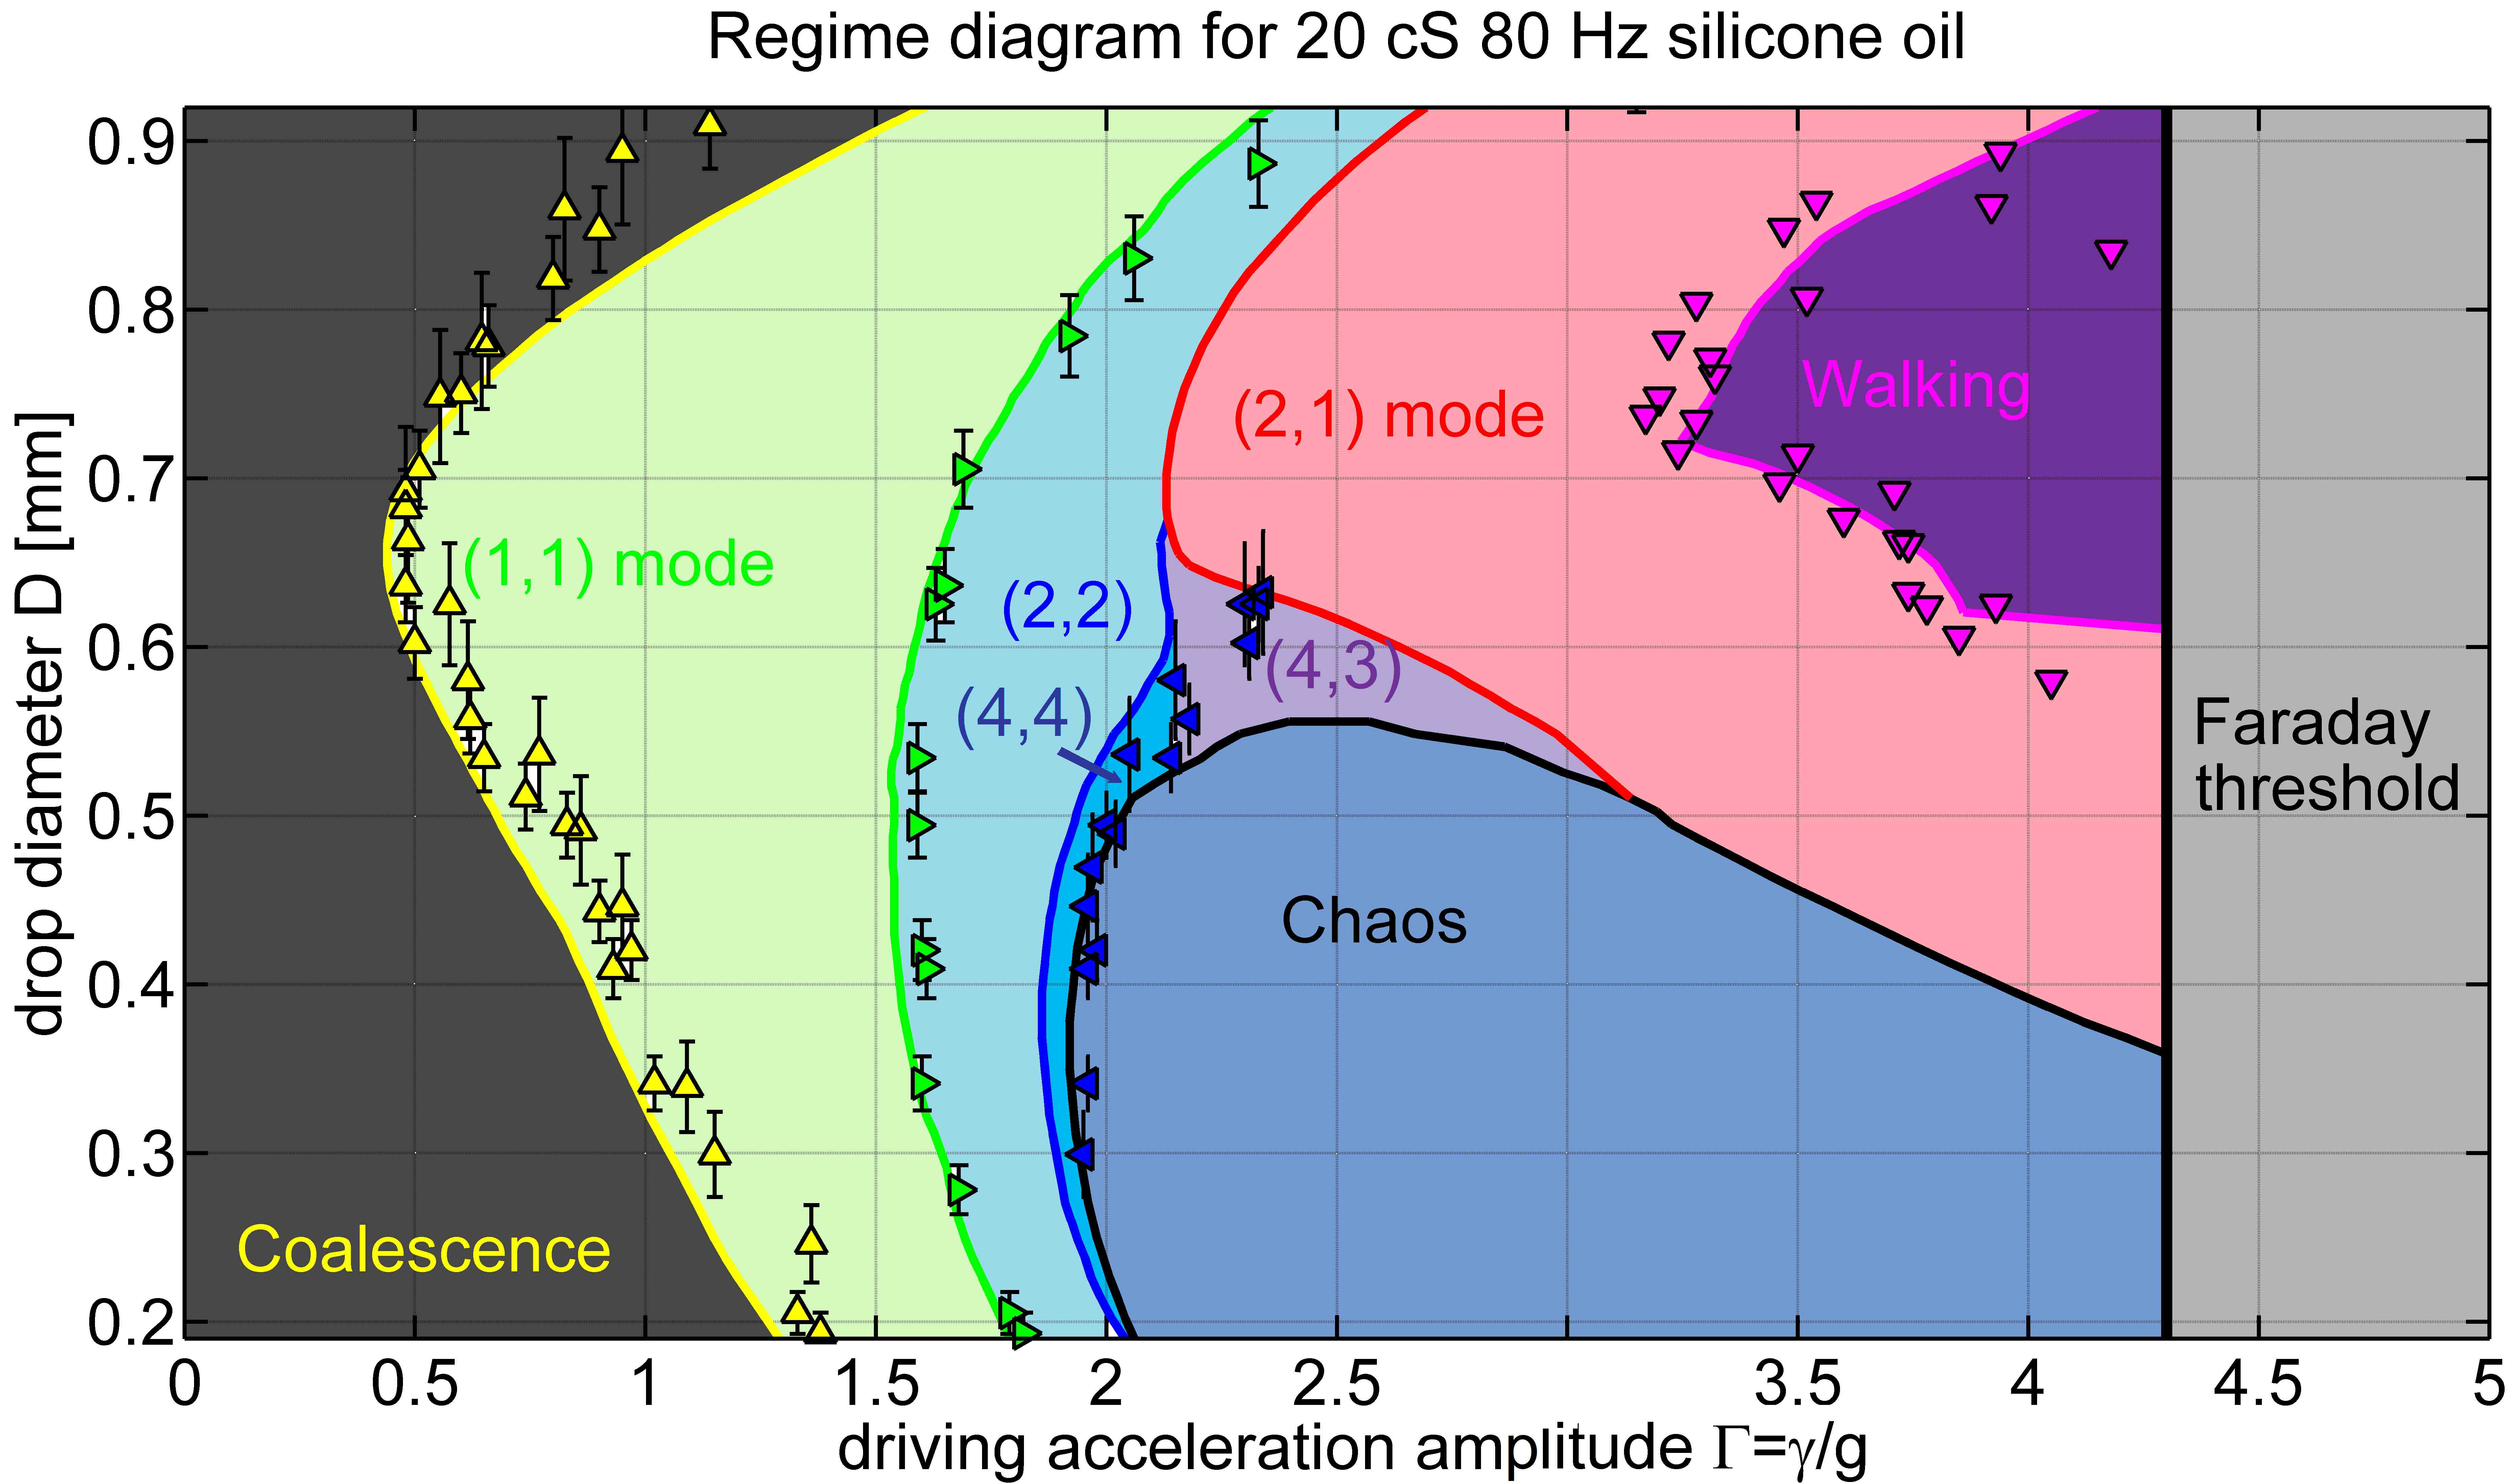
\includegraphics[scale=0.075]{Regime-Mega}
	     \caption{The different bouncing regimes for the oil drops of 20 cS silicon oil and at $f$ = $\omega / 2\pi$ = 80 Hz. The parameters ($m$,$n$) describe the droplet that bounces $n$ times in $m$ forcing periods. }
	 \label{regime}
	\end{figure}

The various modes seen in \refFig{regime} can be described by ($m$,$n$), where $n$ is the number to times the droplet contacts the surface over period $m/f$. For example, in the (1,1) mode, the droplet hits the oil bath once per driving period. In the (2,2) mode, the drop makes two bounces of differing heights. 
	       
            \subsection{Path Memory}
                        
            Path memory is a parameter that can be varied in this setup; it is essentially the damping of the system. Every time the droplet impacts the bath, it creates a radial traveling wave. Over the course of many bounces, a wavefield composed of a superposition of the many waves arises. In this way the wavefield ``remembers" previous interactions. Because droplet motion is influenced by the wavefield, controlling the damping of the wavefield will influence the path of the walker. The heavily damped system has a low memory, while undamped system correspends to higher memory. As one gets closer to the Faraday threshold, one achieves higher and higher memory because waves last for longer. The quantum like features of this experiment arise in the high-memory limit. (For more, Eddi et. al, 2011b: Information stored in Faraday waves.) 
            
             \subsection{Single-Particle Diffraction}
In 2006 Couder and Fort showed that the system had properties that were strikinly similar to two famous and controversial quantum experiments (Couder and Fort, 2006). They were able to demonstrate that a single walker travelling through one slit seemed to have its direction altered seemingly randomly, before continuing forward on its new path. By statistically analyzing many trials, Couder and Fort showed that the histogram of the ``diffraction" actually resulted in a diffraction pattern strikingly similar to the single photon diffraction experiment performed by Taylor in 1909. 

Next, Couder and Fort added a second slit next to the first one. Now a single walker could pass through  one of two slits, and it was discovered that a histomgram of this data returned another diffraction pattern. This result is of course reminiscent of one of the most famous experiments in physics: Young's double slit diffraction with photons and electrons. 
    
Using a numerical simulation, Couder and Fort were able to reproduce similar results. 
    
As Couder and Fort mention in their paper: ``A discussion of the relation between these single-particle experiments and those concerning elementary particles is unavoidable." Important differences and similarities are then described between the quantum system and the quantum-like system. For the differences: we have a dissapative system, where energy is continually put in through the vibration of the tray; the particle can be followed;\footnote{C and F note that it'd be impossible to dectect the particle without disturbing it "by any means at its scale," like a bouy, for example. As the bouy floated it would interfere with the system by altering the wave pattern on the surface.} it's really effectively moving in two dimensions; the velocity is measurable; and the probability distributuion is linked with the wave amplitude (rather than it's intensity). And then of course, the similarities: an uncertainty priciple arises from the statistical data (and without knowledge of the actual paths followed by the walkers); and some others that were unclear...

Recently, Harris attempted to reproduce single slit interference. With better technology, new results were found. Using a looping guiding batt, trajectories were found to follow the same loop without deviating. Only at a very high memory were there chaotic paths.


\subsection{Tunneling}
	       The guiding wave field can be partially reflected off of an edge or even a change in depth of the oil bath. This effect can be seen when a walker is pushed back from a under-the-surface step, seemingly without any contact. In rare cases, the walker will actually tunnel across the step; that is, it will continue to walk along the surface of the oil bath and pass over the step without reflection. In the first experiment done by Eddi et al., they demonstrated tunneling by by building square ``corrals" of varying thicknesses. In the second experiment, they built a rhombus shape which forced the walker across the center of a rhombus. The barrier was placed perpendicular to the direction of travel of the walker, so that it would hit the wall directly rather than at an angle (as in the square corral). ``The tunneling probability decreases exponentially with the barrier width and increases as the Faraday threshold is approached." Eddi et. al also found that the probability of tunneling increased with the velocity of the walker. (For more, Eddi et. al 2009b: Unpredictable Tunneling of a classical wave-particle association.)
	       
	       
	        The unpredictability of the tunneling comes from the complex interatction between the drop and its guiding wave. 


